\section{Question Pattern Identification in Existing KGQA Benchmarks}\label{sec:kbqa_benchmark_appendix}

\subsection{Introduction of Existing KGQA Benchmarks}

As listed in~\autoref{tab:benchmark_comparison}, there are seven major KGQA benchmarks developed over the past decade. Specifically, SimpleQ~\cite{simpleq} and WebQSP~\cite{webqsp} are two early KGQA benchmarks. SimpleQ constructs queries from Freebase facts by using the subjects and relationships as inputs and treating the objects as answers, which means it only contains questions of the $\langle s,p,* \rangle$ type in our taxonomy (discussed below). WebQSP is derived by selecting only those questions from WebQuestions~\cite{webquestion} that can be translated into simple SPARQL queries; the original questions in WebQuestions were generated using the Google Suggest API~\cite{googlesuggestapi}. To verify the question patterns in WebQSP, we prompt the LLM to analyze the queries and validate that most of the questions in WebQSP also belong to the $\langle s,p,* \rangle$ pattern. CWQ~\cite{cwq}, GraphQ~\cite{graphq}, and GrailQA~\cite{grailqa} are more recent benchmarks that feature higher query complexity. CWQ builds upon WebQSP by applying additional fact constraints (e.g., conjunctions and compositions) to the original SPARQL queries. GraphQ and GrailQA employ a graph-expansion algorithm to induce a subgraph from the question entity and then generate a question based on each subgraph. Although these datasets contain questions with multiple fact constraints and include features like counting, superlatives (e.g., argmax, argmin), and comparatives, the questions still ask about a concrete entity and can largely be categorized as combinations of $\langle s,p,* \rangle$ patterns.

\subsection{Question Patterns in Existing KGQA Benchmarks}

\begin{table}[ht]
\centering
\caption{Number of questions of each question pattern in WebQSP, CWQ and WIKIQA.}
\label{tab:benchmark_question_pattern}
\resizebox{0.9\textwidth}{!}{%
\begin{tabular}{@{}cccccccccc@{}}
\toprule
\multirow{3}{*}{\textbf{Benchmark}} & \multicolumn{4}{c}{\textbf{basic Question Pattern}} & \multicolumn{4}{c}{\textbf{Nested Question Pattern}} \\ \cmidrule(lr){2-9}
 & \multirow{2}{*}{$\langle s,*,* \rangle$} & \multirow{2}{*}{$\langle s,p,* \rangle$} & \multirow{2}{*}{$\langle s,*,o \rangle$} & \multirow{2}{*}{$\langle s,p,o \rangle$} & $\langle s,*,* \rangle$ & $\langle s,p,* \rangle$ & $\langle s,*,o \rangle$ & $\langle s,p,o \rangle$ &  \\
 &  &  &  &  & $\langle s,p,* \rangle$ & $\langle s,p,* \rangle$ & $\langle s,p,* \rangle$ & $\langle s,p,* \rangle$ &  \\ \midrule
WebQSP~\cite{webqsp} (2016) & 179 & 4,558 &  &  &  &  &  & \\
CWQ~\cite{cwq} (2018) &  & 19,631 &  &  &  & 15,058 &  & \\ 
WIKIQA~\cite{wikiqa} (2015) & 761 & 1,753 & 276 & & 24 & 224 & & \\ \bottomrule
\end{tabular}%
}
\end{table}

For most benchmarks, the question pattern can be inferred from their question generation procedures—for example, from the templates used in RGBench~\cite{graphcot} and CypherBench~\cite{cypherbench}, or the subgraph construction methods in GraphQ~\cite{graphq} and GrailQA~\cite{grailqa}. However, for WebQSP~\cite{webqsp} and CWQ~\cite{cwq}, we need to examine the questions directly to determine their corresponding patterns, as these questions are generated using the Google Suggest API. To this end, we classify each question in WebQSP and CWQ using an LLM (Claude-3.5-sonnet). The prompt used to guide the LLM in identifying the question pattern is largely the same as the one used in \name{} for question categorization, as shown in~\autoref{fig:qc_prompt}. This prompt provides clear definitions of each question pattern, includes concrete few-shot examples, and allows for exceptions where questions do not fit cleanly into one of the four basic patterns and should instead be labeled as nested questions. Additionally, we ask the LLM to provide a question decomposition for each nested question. In the following, we discuss the question categorization results of WebQSP and CWQ, respectively.

\autoref{tab:benchmark_question_pattern} reports the results on WebQSP and CWQ. We observe that the majority of questions in the WebQSP benchmark fall into the $\langle s,p,*\rangle$ pattern, with only 179 out of 4,737 questions belonging to the $\langle s,*,* \rangle$ category. An example of a $\langle s,*,* \rangle$ question is “What is Mount St. Helens?”. Although such questions typically lack definitive ground-truth answers, WebQSP annotates responses like “Stratovolcano” and “Volcano”, which reduces the evaluation to checking for the presence of certain keywords rather than assessing the overall quality or helpfulness of the information. There are no $\langle s,*,o \rangle$ or $\langle s,p,o \rangle$ questions in WebQSP, as it is difficult to define a unique set of ground-truth answers for these types. In contrast, CWQ~\cite{cwq}, which is sampled and augmented from WebQSP, introduces additional $\langle s,p,* \rangle + \langle s,p,* \rangle$ questions by incorporating extra fact constraints using conjunctions, superlatives, comparatives, and compositions. This results in 15,058 nested $\langle s,p,* \rangle + \langle s,p,* \rangle$ questions out of the total 34,689 questions.


To study the diversity and possible graph question patterns that may arise in real-world scenarios, we analyze WIKIQA~\cite{wikiqa}, a text-understanding benchmark whose questions are extracted from real Bing query logs. We apply the same classification method used for WebQSP and CWQ to determine the pattern of each question in WIKIQA. As reported in~\autoref{tab:benchmark_question_pattern}, among the 3,047 questions, 761 fall under the $\langle s,*,* \rangle$ pattern, 1,753 under $\langle s,p,* \rangle$, and 276 under $\langle s,*,o \rangle$. Among the nested questions, 24 follow the $\langle s,*,* \rangle + \langle s,p,* \rangle$ pattern and 224 follow $\langle s,p,* \rangle + \langle s,p,* \rangle$. No $\langle s,p,o \rangle$ questions are found in WIKIQA, likely because the dataset only includes question-like queries that begin with WH-words (e.g., “what” or “how”) and end with a question mark. In contrast, $\langle s,p,o \rangle$ questions are more likely to start with expressions such as “Is there,” “Do,” or “Have.” Furthermore, since WIKIQA extracts only a subset of Bing query log data using basic word filtering, its question pattern distribution may not fully represent real-world scenarios. Nonetheless, the presence of multiple question patterns in WIKIQA supports the validity of our proposed taxonomy.


\begin{figure*}[!h]
	\centering
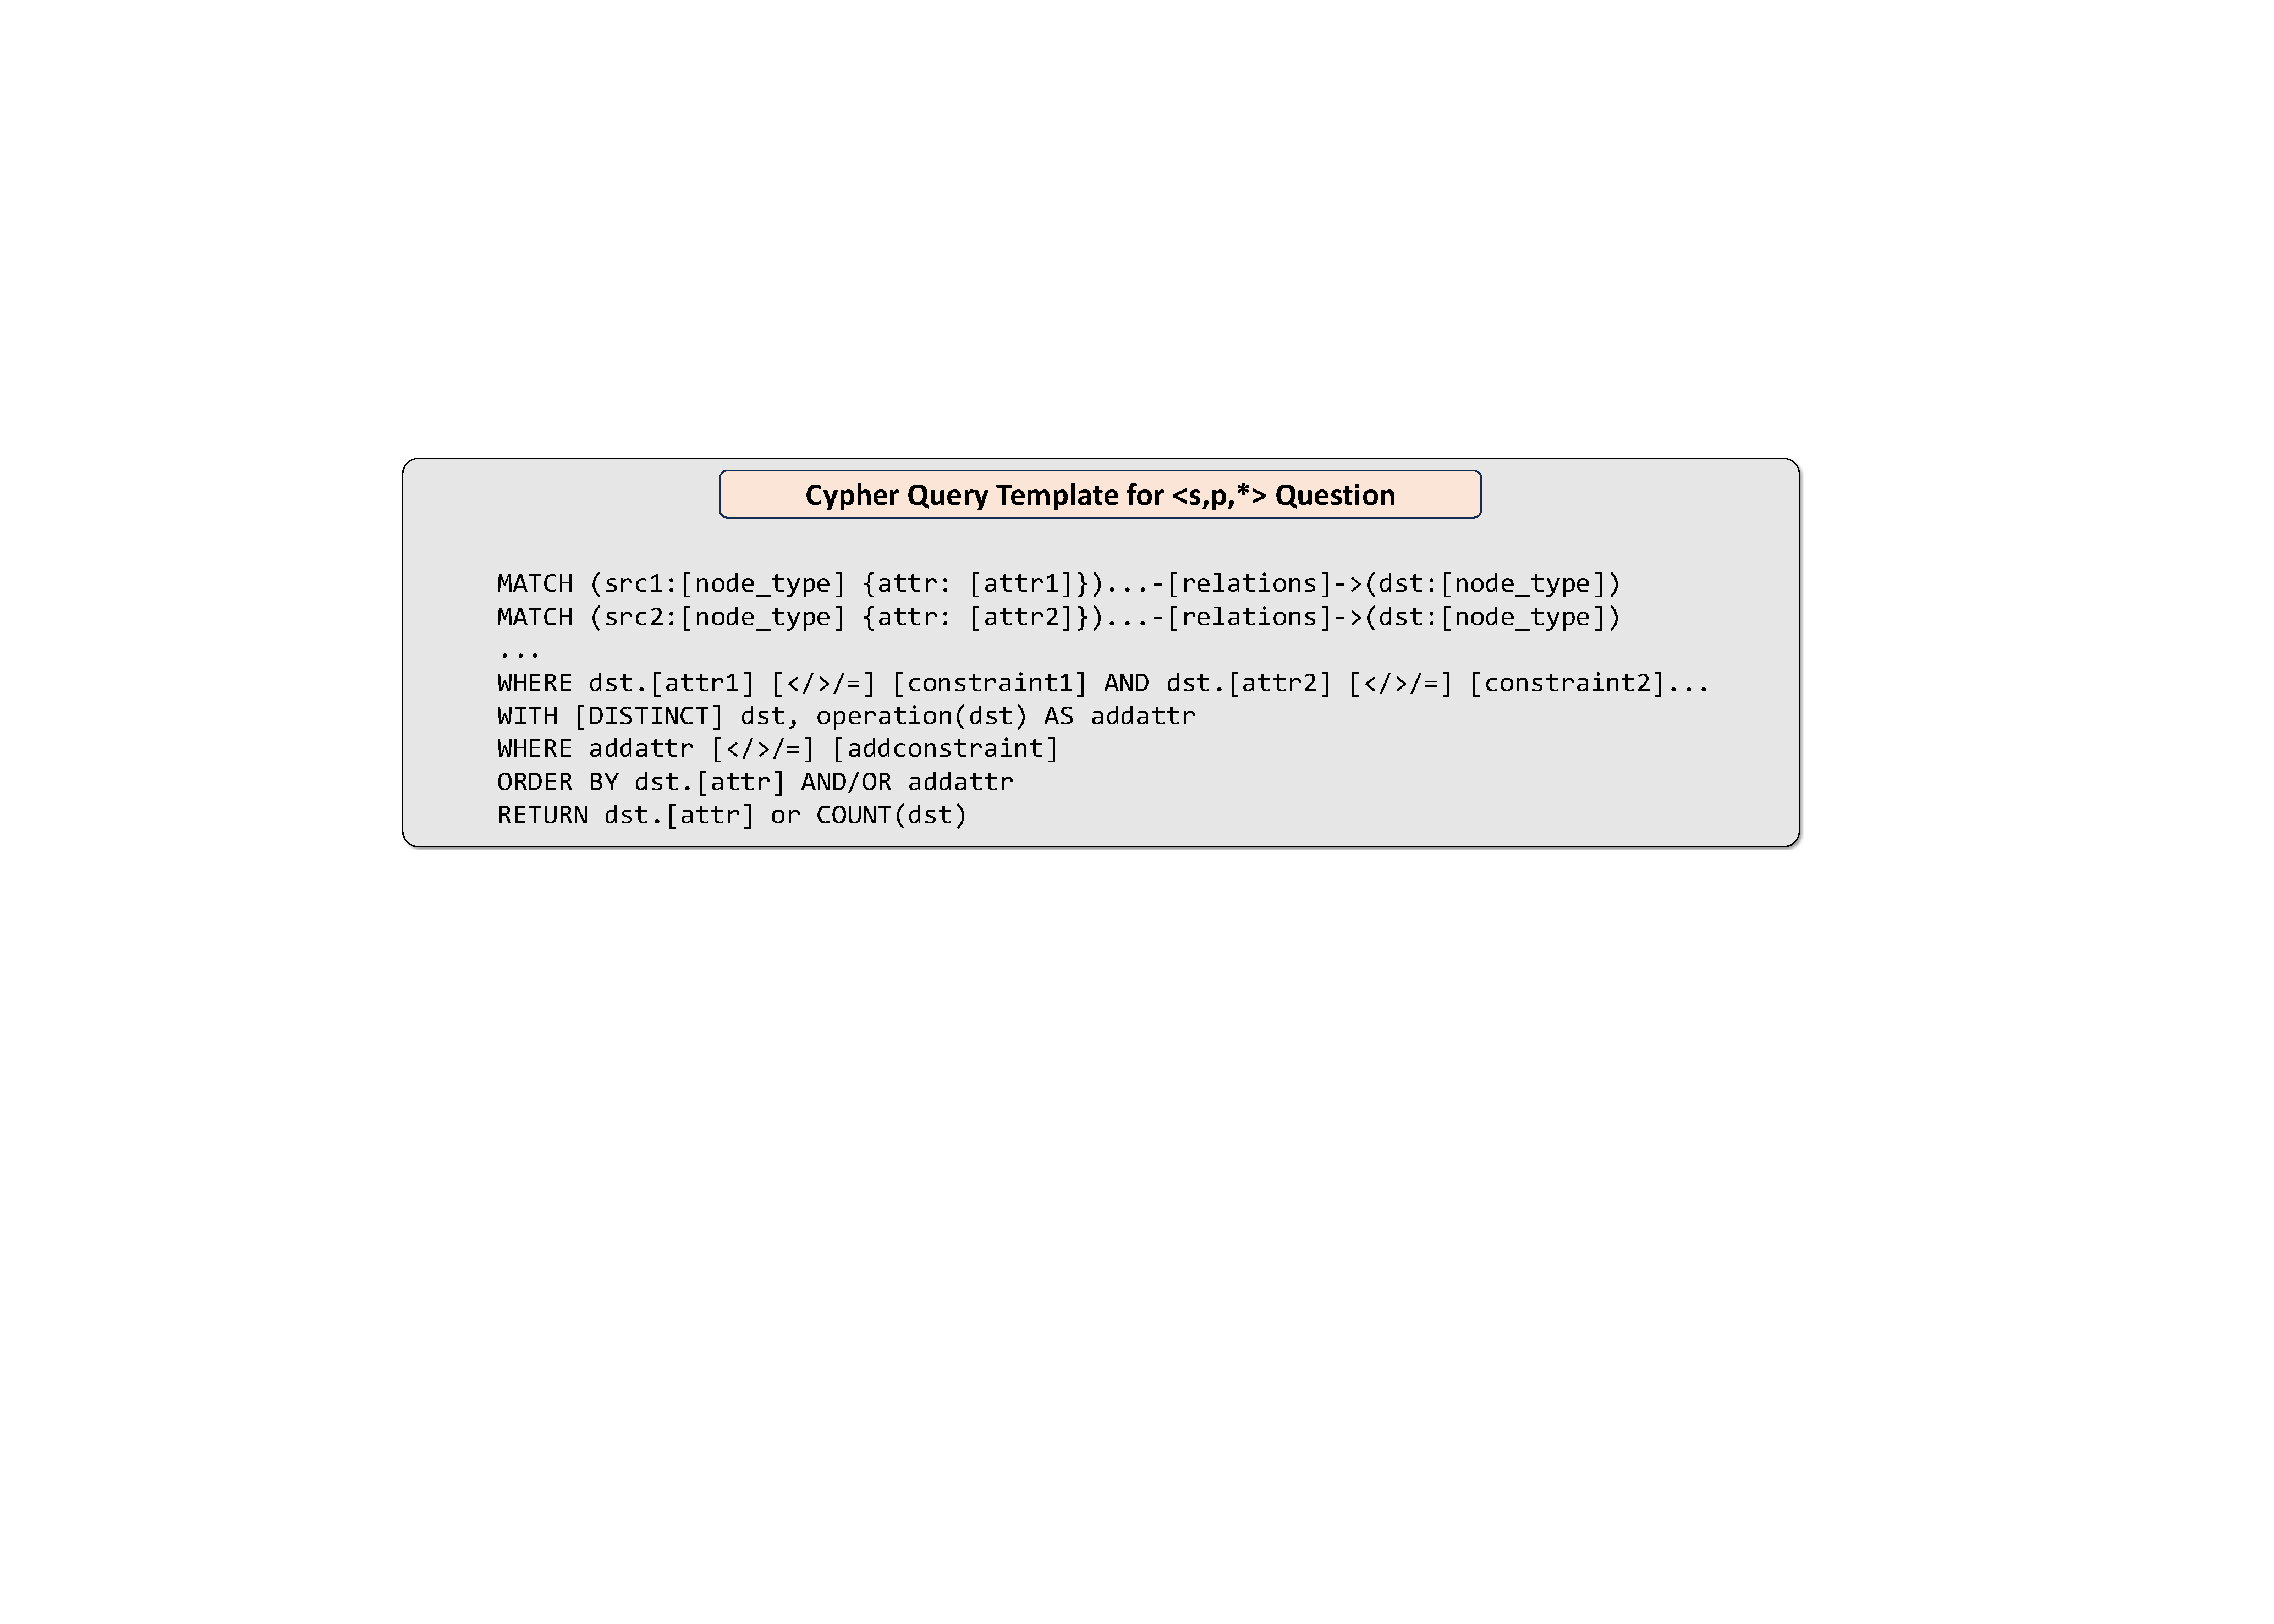
\includegraphics[width=\textwidth]{figures/appendix/cypher_template.pdf}
	% \vspace{-4mm}
	\caption{Cypher template for $\langle s,p,* \rangle$ questions.}
	\label{fig:cyper_template}
	 % \vspace{-2mm}
\end{figure*}

As we have established, most existing KGQA benchmarks primarily contain questions following the $\langle s,p,* \rangle$ pattern and its nested extension $\langle s,p,* \rangle + \langle s,p,* \rangle$. We now illustrate how representative questions from these benchmarks exhibit strong similarities and limit the diversity of question coverage. In particular, we observe that they share similar Cypher query structures for retrieving the desired answers, which can be abstracted into a general template, as shown in~\autoref{fig:cyper_template}. Empirically, all $\langle s,p,* \rangle$ questions can be instantiated using this Cypher template, with the specific graph schema guiding how the relations in the graph correspond to the fact constraints expressed in the user question. Below, we present several examples to demonstrate how this template can be instantiated for various $\langle s,p,* \rangle$ questions.


\circled{1} \textit{"Which city held the summer Olympics twice?"}

Cypher query:

\begin{lstlisting}[style=cypher, language=]
MATCH (src:[Event] {name: [Summer Olympics]})-[held in]->(dst:[City])
WITH DISTINCT dst, COUNT(dst) AS count
WHERE count == 2
RETURN dst.name
\end{lstlisting}

\circled{2} \textit{"What year did the Florida Marlins win their 2nd world series title?"}

Cypher query:

\begin{lstlisting}[style=cypher, language=]
MATCH (src:[Title] {name: [World Series Chaimpion]})-[rel:won by]->(dst:[Team])
WHERE dst.name == Florida Marlins
WITH dst, src
ORDER BY src.date
RETURN dst.name
LIMIT 1
\end{lstlisting}

\circled{3} \textit{"Which states does the river that flows under the DeSoto Bridge pass through?"}

Cypher query:

\begin{lstlisting}[style=cypher, language=]
MATCH (src:[Bridge] {name: [DeSoto Bridge]})-[on top of]->(n:[River])-[pass through]->(n:[City])-[belong to]->(dst:[States])
WITH DISTINCT dst
RETURN dst.name
\end{lstlisting}

\circled{4} \textit{"How many languages are used where \"Lupang Hinirang\" is the national anthem?"}

Cypher query:

\begin{lstlisting}[style=cypher, language=]
MATCH (src:[Song] {name: [Lupang Hinirang]})-[national anthem]->(n:[Country])-[people]->(n:[People])-[speak]->(dst:[Language])
WITH DISTINCT dst
RETURN COUNT(dst)
\end{lstlisting}
